\documentclass[a4paper,11pt]{article}
\usepackage[utf8]{inputenc}
\usepackage{kotex}
\usepackage{geometry}
\usepackage{lipsum}
\usepackage{setspace}
\usepackage{sectsty}
\usepackage{graphicx}
\usepackage{subcaption}
\usepackage{algorithm}
\usepackage{algorithmic}
\usepackage{pdfpages}
\usepackage{titlesec}
\usepackage{tocloft}
% \usepackage{hyperref}
% \usepackage{bookmark}
% \usepackage{fontspec}

\titleformat{\section}[block]{\normalfont\Large\bfseries\filcenter}{제 \thesection\ 장}{1em}{}
\renewcommand{\thesection}{\arabic{section}}
% \usepackage{subfig}

\sectionfont{\fontsize{16}{19}\selectfont}
\subsectionfont{\fontsize{13}{16}\selectfont}

\doublespacing  
\geometry{ top=38mm, bottom=37mm, left=35mm, right=35mm}

\renewcommand{\abstractname}{}
\renewcommand{\refname}{\centering 참고문헌}

\renewcommand{\contentsname}{\centering 차례}
\renewcommand{\listfigurename}{\centering 그림 목차}

\renewcommand{\cftsecleader}{\cftdotfill{\cftdotsep}}
\renewcommand{\cftsecfont}{\bfseries}
\renewcommand{\cftsecpagefont}{\normalfont}
\renewcommand{\cftsecpresnum}{제\ }
\renewcommand{\cftsecaftersnum}{장}
\renewcommand{\cftsecnumwidth}{3.5em}
\renewcommand{\cftsecindent}{1.5em}


\title{트랜잭션 실행 간 탈중앙성 강화를 위한 이더리움 네트워크의 트랜잭션 실행 보장 구조 설계}
\author{[서상원]} 
\date{[2023.10.20.]}

\begin{document}

\includepdf[pages=1-2]{including/front.pdf}
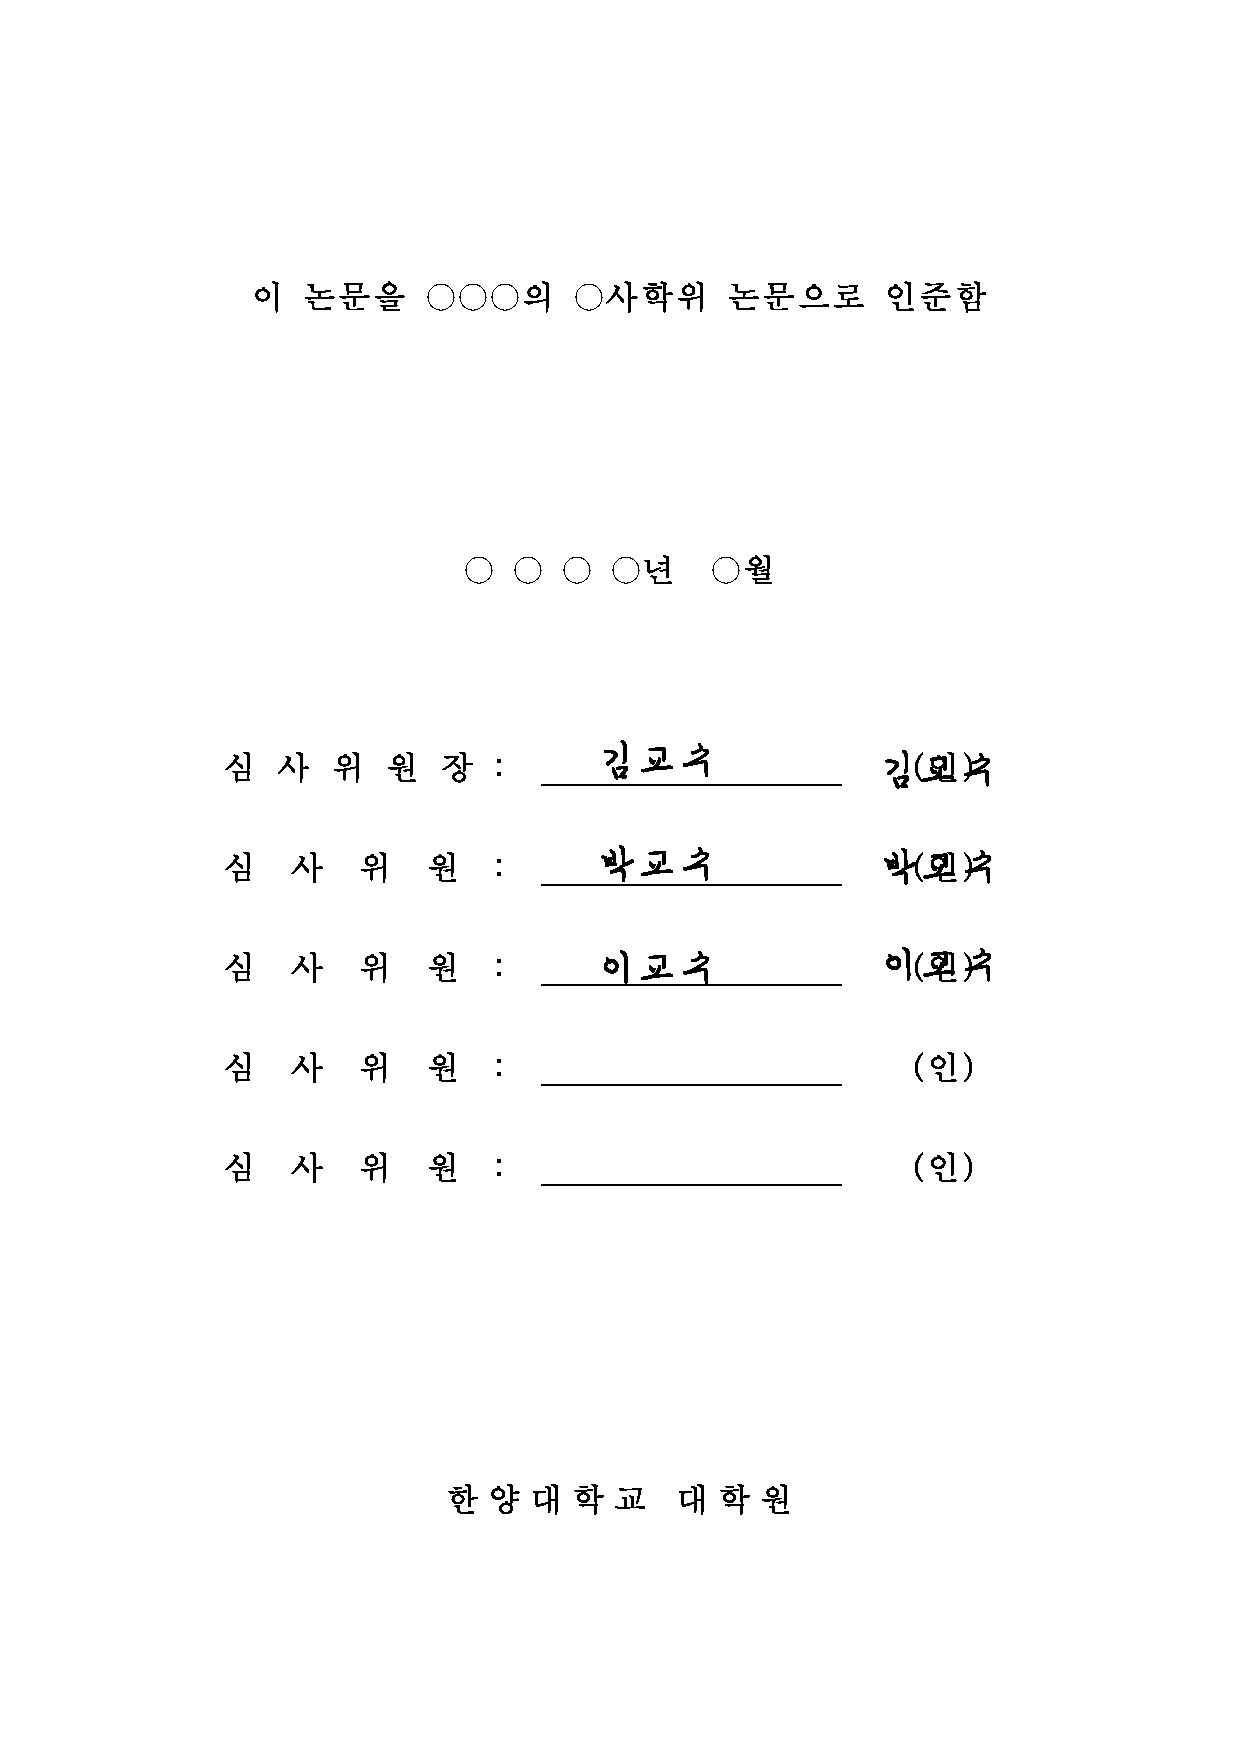
\includepdf[pages=-]{including/stamps.pdf}

\newpage 
\pagenumbering{roman} % 서론 부분에 로마 숫자 페이지 번호 사용

\setcounter{page}{1}
\tableofcontents

\newpage
\clearpage % 페이지 분리 
\section*{\centering 국문 요지} % Abstract 섹션, 번호 없음
\addcontentsline{toc}{section}{국문 요지} % Abstract를 목차에 추가

% \maketitle
\begin{abstract}
    본 연구는 [연구 주제]에 대해 다루고 있으며, [연구의 목적 또는 필요성]을 탐구한다. 
    이 연구에서는 [연구 방법론]을 사용하여 [연구 대상 또는 데이터]을 분석하였다. 
    연구 결과, [주요 발견 또는 결과]가 도출되었으며, 이는 [연구 분야의 기존 지식이나 이론]에 대한 중요한 시사점을 제공한다. 
    또한, [연구의 한계점 및 향후 연구 방향]에 대해서도 논의하였다. 
    본 논문은 [해당 분야]의 전문가 뿐만 아니라 관련 분야의 학생들에게도 유용한 정보와 인사이트를 제공할 것으로 기대된다.
\end{abstract}
% \newpage
% \tableofcontents
\newpage
\addcontentsline{toc}{section}{그림 목차} % Abstract를 목차에 추가

\listoffigures
\newpage
\pagenumbering{arabic} % 본문에 아라비아 숫자 페이지 번호 사용
\setcounter{page}{1}

\section{서론}

본 연구는 [연구 주제에 대한 간략한 소개]를 다루고 있다. [연구 주제의 배경 및 현황]을 간략히 설명하고, 이와 관련된 기존 연구들의 주요 발견 및 한계점을 언급한다. 이러한 배경을 토대로, 본 논문은 [연구가 다루고자 하는 주요 문제점 또는 질문]에 초점을 맞추고 있다.

본 논문의 주요 목적은 [연구의 목적 또는 연구가 해결하고자 하는 문제]를 명확히 밝히는 것이다. 이를 통해 [연구의 기대 효과 또는 기여도]를 설명하고, [해당 연구 분야에 대한 연구의 중요성]을 강조한다.

이 연구는 [연구 방법론 및 접근 방식]을 채택하여 [연구 진행 과정의 간략한 개요]를 제공한다. 본 연구의 결과는 [해당 분야의 학계나 실무에 어떤 영향을 미칠지에 대한 논의]를 포함한다.

이 서론은 연구의 배경을 설정하고, 연구의 목적과 중요성을 강조하며, 본 논문의 구조에 대한 개요를 제공함으로써 독자가 본문 내용을 보다 잘 이해할 수 있도록 돕는다.

\newpage

\section{관련연구}
이 장에서는 [연구 주제]와 관련된 기존 연구들을 검토한다. 
이 검토는 [연구 분야]에 대한 이해를 깊게 하고, 본 연구가 기존 연구와 어떻게 차별화되는지를 명확히 하는 데 목적이 있다.
인용은 이 줄을 따라서 하면 된다.\cite{buterin2014next,wood2014ethereum}

\subsection{[첫 번째 하위 주제 또는 연구 분야]}
[첫 번째 하위 주제 또는 연구 분야]에 대한 기존 연구들을 검토한다. 
이 부분에서는 [해당 분야의 주요 연구 결과 및 주장들]을 소개하고, 이들이 본 연구와 어떻게 연결되는지 논의한다.

\subsection{[두 번째 하위 주제 또는 연구 분야]}
둘째, [두 번째 하위 주제 또는 연구 분야]에 대해 논의한다. 
이 부분에서는 [해당 분야에서 나타난 중요한 경향 및 발전]을 분석하고, 본 연구의 맥락에서 이들의 중요성을 평가한다.

\subsection{[기존 연구들의 한계점 및 본 연구가 이를 어떻게 해결하고자 하는지]}
셋째, [기존 연구들의 한계점 및 본 연구가 이를 어떻게 해결하고자 하는지]에 대해 설명한다. 
이는 본 연구의 필요성과 중요성을 강조하는 데 중요한 역할을 한다.

\subsection{[기존 연구들의 검토를 바탕으로 한 본 연구의 독창성 및 기여도]}
본 장의 결론에서는 [기존 연구들의 검토를 바탕으로 한 본 연구의 독창성 및 기여도]를 강조한다.



\newpage

\section{본문}
본문은 그냥 쓰시면 됩니다.

\subsection{이미지 첨부 방법}
\begin{figure}[h]
    \centering
    
\includegraphics[width=0.75\linewidth]{figure/1.png}
    \caption{First Image}
    \label{fig:firstImage}
\end{figure}
이미지는 이렇게 Figure \ref{fig:firstImage} 가져다가 쓸 수 있다.
이미지 번호는 그냥 알아서 해준다.



\subsection{수도코드 첨부 방법}
수도코드는 아래처럼 하면 된다.

\begin{algorithm}
    \caption{Your Algorithm Name}
    \label{alg:your_algorithm}
    \begin{algorithmic}[1] % The number tells where the line numbering should start
        \REQUIRE $n \geq 0 \vee x \neq 0$ % Input requirements
        \ENSURE $y = x^n$ % Output specifications
        \STATE $y \leftarrow 1$
        \STATE $X \leftarrow x$
        \STATE $N \leftarrow n$
        \WHILE{$N \neq 0$}
            \IF{$N$ is even}
                \STATE $X \leftarrow X \times X$
                \STATE $N \leftarrow N / 2$ 
            \ELSE[$N$ is odd]
                \STATE $y \leftarrow y \times X$
                \STATE $N \leftarrow N - 1$
            \ENDIF
        \ENDWHILE
    \end{algorithmic}
\end{algorithm}

\newpage   
\clearpage % 페이지 분리 

\section{결론}
본 논문은 [연구 주제]에 대한 포괄적인 연구를 수행하였으며, 이 과정에서 여러 중요한 발견을 하였다. 
주요 발견으로는 [주요 발견 1], [주요 발견 2] 및 [주요 발견 3] 등이 있다. 
이러한 발견들은 [연구 분야]에 대한 이해를 심화시키고, [연구 분야의 특정 문제나 질문에 대한 새로운 통찰]을 제공한다.

이 연구는 [연구 방법론의 효율성 및 적절성]에 대해서도 중요한 시사점을 제공한다. 
[연구 방법론]의 사용은 [특정 유형의 데이터나 현상을 이해하는 데 유용함]을 입증하였다.

그러나 본 연구는 몇 가지 한계점을 가지고 있다.
이러한 한계점은 [한계점 1], [한계점 2] 등으로, 이는 향후 연구에서 해결해야 할 과제들을 시사한다. 
따라서, 향후 연구에서는 [향후 연구 방향 1], [향후 연구 방향 2] 등의 주제를 탐구하는 것이 바람직하다.

종합적으로 볼 때, 본 연구는 [연구 분야]에 대한 심도 있는 이해를 제공하며, 향후 연구자들에게 유용한 기초를 마련해 준다. 
본 연구의 발견과 제안은 [연구 분야]의 발전에 기여할 것으로 기대된다.


\newpage 

\addcontentsline{toc}{section}{참고문헌} 

\bibliographystyle{unsrt}
\bibliography{references}
\newpage
\section*{\centering ABSTRACT}
\subsection*{\centering [ENGLISH PAPER]}

\addcontentsline{toc}{section}{ABSTRACT}
\begin{flushright}
HONG, GIL DONG\\[-0.5em]
Dept. of Yours\\[-0.5em]
Graduate School of\\[-0.5em]
Hanyang University
\end{flushright}
\begin{abstract}
    This study explores [the main topic of the research] and aims to [state the primary objective of the research]. 
    Utilizing [briefly describe the methodology], the research examines [specify the subject or data of the research]. 
    The key findings include [list the main results or discoveries], which offer significant insights into [mention the broader field or implications of the research].
    Furthermore, the research addresses [any specific aspects or secondary objectives of the study]. 
    The results demonstrate [describe the outcome of the research in relation to the objectives]. 
    These findings contribute to [mention how the research contributes to the existing knowledge or practice in the field].
    The study also discusses [note any limitations of the research and potential areas for future research]. 
    Overall, this research provides valuable perspectives on [restate the main topic or field], and it is anticipated to be a beneficial resource for professionals and students in [mention the relevant field or discipline].
\end{abstract}

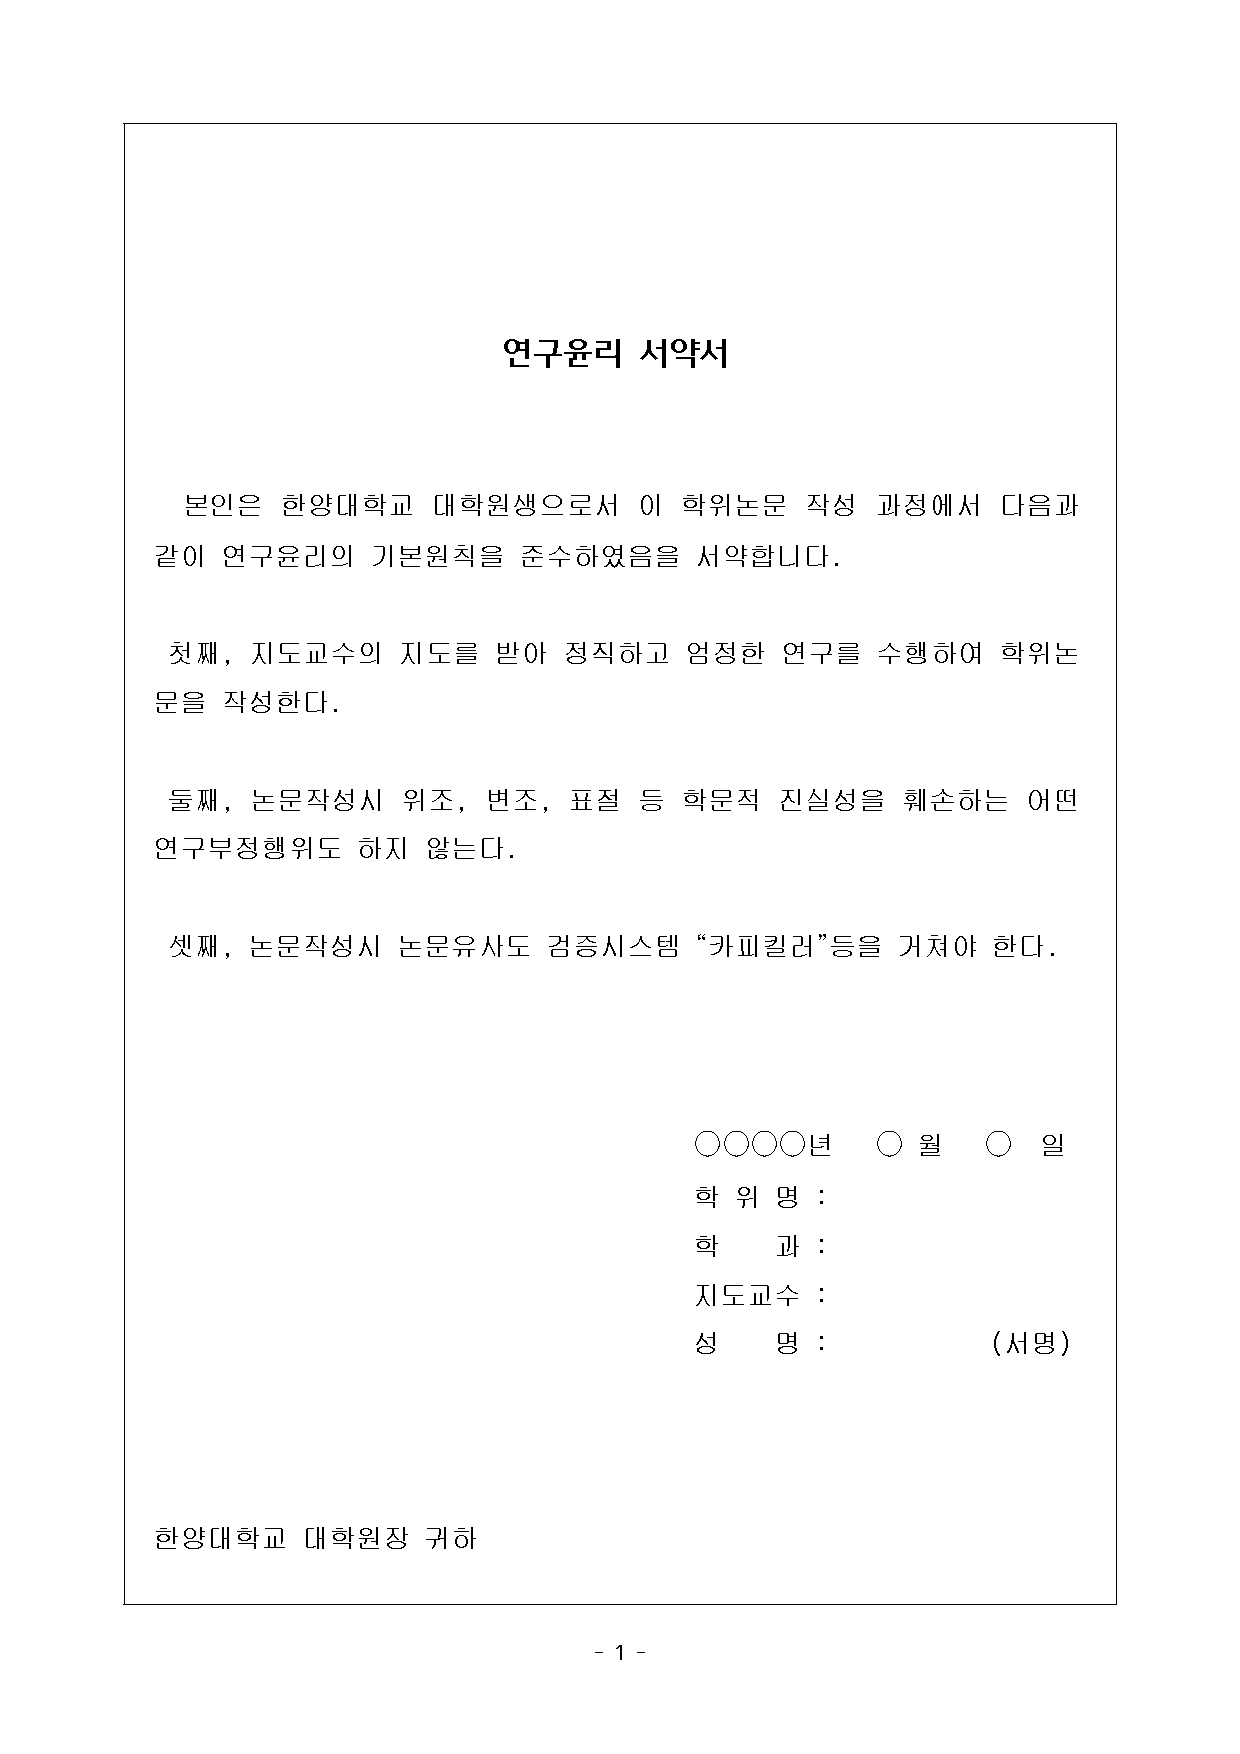
\includepdf[pages=-]{including/sign.pdf}

\end{document}